To prepare the data several preprocessing operations were performed:

\vspace{0.2cm}\noindent
\textbf{Noise Reduction:} the audio data was already provided in a clipped format 
to minimize noise and irrelevant information.

\vspace{0.2cm}\noindent
\textbf{Normalization}: the audio are loaded using the \textit{torchaudio.load()} 
function, which normalized the audio signals in the range [-1, 1]. 

\vspace{0.2cm}\noindent
\textbf{Removal of Corrupted Files:} corrupted files were identified and removed 
from the dataset to ensure data quality.

\vspace{0.2cm}\noindent
\textbf{Outlier Detection and Removal:} we investigated the average duration of 
each class and found the 'artifact' class to have a significantly larger average 
duration. This was due to a few long lasting audio 
recordings (see Figure \ref{fig:DataExp_outliers_Artifacts}). A large number of samples from 
the same audio might not be as informative, thereby we used IQR to detect and remove outliers.

\vspace{0.2cm}\noindent
\textbf{Resampling:} we evaluated two sampling rates to determine the optimal rate 
for heartbeat sounds and all audio files were resampled to a common frequency of 4000 Hz 
(see Section \ref{sec:sampling_rate}).

\vspace{0.2cm}\noindent
\textbf{Segmentation:} the audio data was segmented into 1-second intervals, 
identified as the optimal extraction interval (see Section \ref{sec:extraction_interval}), as
it offered both good performance and dataset size increasing.

\vspace{0.2cm}\noindent
\textbf{Hop and Window Size}: the hop size determines the number of samples between 
successive windows, while the window size determines the number of samples considered. 
Each feature was extracted using the same window length and hop length facilitating a 
fair assessment of each feature's contribution to the classification task. 

\begin{figure}[H]
	\centering
	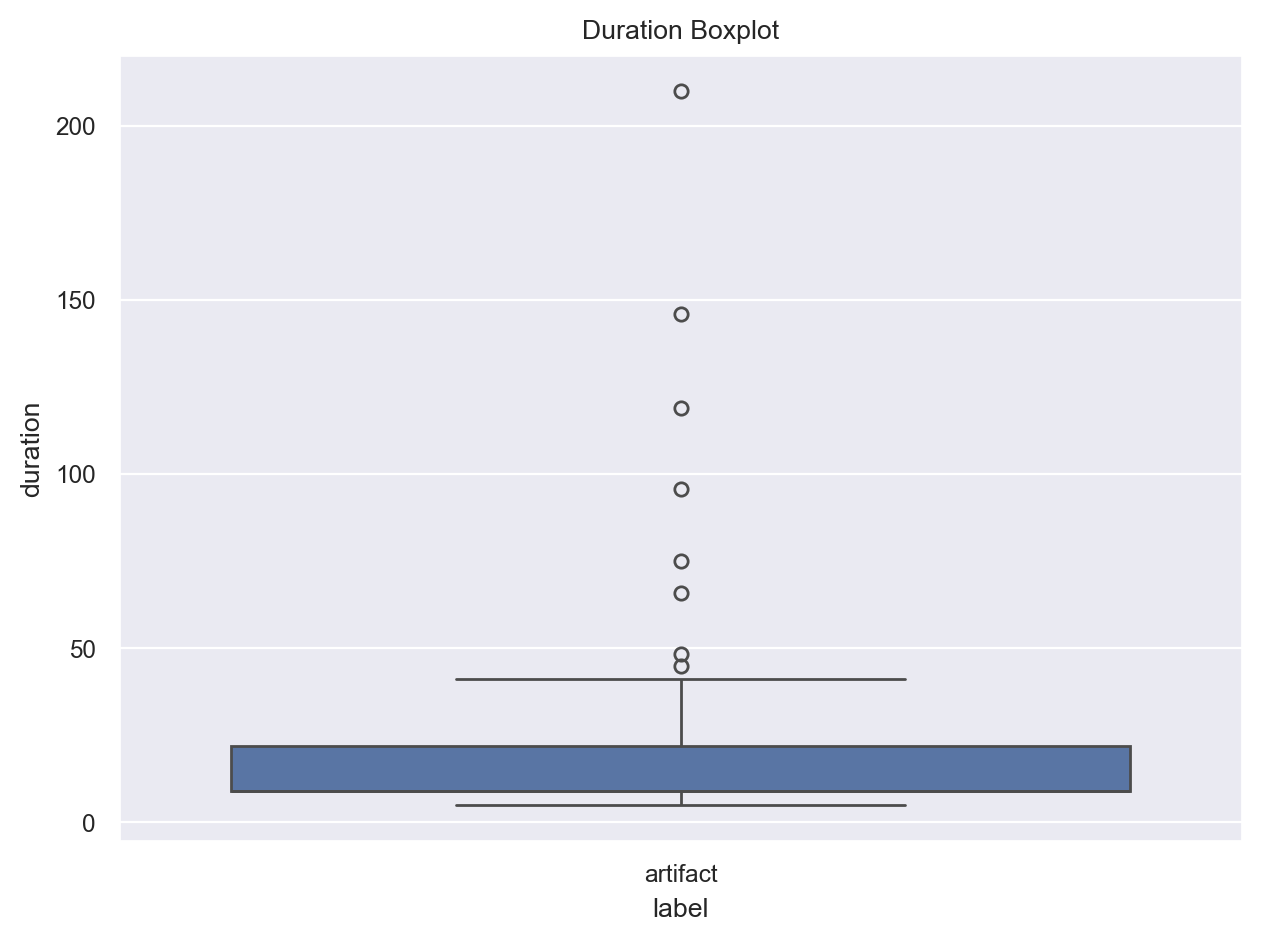
\includegraphics[width=1\columnwidth]{./images/DataExp_outliers_artifact.png}
	\caption{Outliers in the Artifacts class.}
	\label{fig:DataExp_outliers_Artifacts}
 \end{figure}\subsection{Data Preprocessing}
